\documentclass[tikz,border=10pt]{standalone}
\begin{document}
  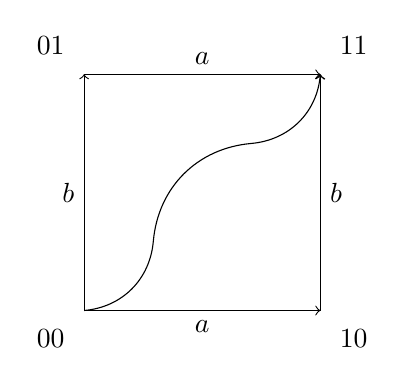
\begin{tikzpicture}[node distance=3cm, align=center]
    \title{a transition system}

    \node(q1) [label=below left:{$00$}]            {};
    \node(q2) [above of=q1, label=above left:{$01$}]    {};
    \node(q3) [right of=q1, label=below right:{$10$}]    {};
    \node(q4) [right of=q2, label=above right:{$11$}]    {};
    
    \node(q11) [below left of=q4] {};
    \node(q12) [above right of=q1] {};
    
    %\draw [->][draw=black] (q1.center) to [out =40,in =110] node {} (q11.center) to [out=-70,in=-150] (q4.center);
    \draw [->][draw=black] (q1.center) to [bend right=40] (q11.center) to [bend left] (q11.center) to [bend left=40] (q12.center) to [bend right=40] (q4.center);
%    \draw [->][draw=black] (q1.center) to [out=70,in=110] node {} (q11.center) to [out=-70, in=-150] (q4.center);
    
    \draw [->][draw=black] (q1.center) to node [left] {$b$} (q2.center);
    \draw [->][draw=black] (q1.center) to node [below] {$a$} (q3.center);
    \draw [->][draw=black] (q2.center) to node [above] {$a$} (q4.center);
    \draw [->][draw=black] (q3.center) to node [right] {$b$} (q4.center);


  \end{tikzpicture}
\end{document}